\documentclass[12pt,a4paper,twoside]{article}



% Consolidated submission source generated from the modular Draft 1 project.

% Edit the modular project files for future revisions; regenerate this file for submission.

% ==================== EMBEDDED ZOTERO BIBLIOGRAPHY ====================
\begin{filecontents*}{ELL305-Draft-1-references.bib}
@report{amd2022epyc7003,
  title = {{{AMD EPYC}} 7003 Processor Microarchitecture Overview},
  author = {{Advanced Micro Devices, Inc.}},
  date = {2022},
  number = {57075},
  institution = {Advanced Micro Devices, Inc.},
  url = {https://www.amd.com/content/dam/amd/en/documents/epyc-technical-docs/white-papers/overview-amd-epyc7003-series-processors-microarchitecture.pdf},
  keywords = {AMD,draft-1,ELL305,EPYC,Zen 3}
}

@inproceedings{naffziger2020chiplet,
  title = {{{AMD}} Chiplet Architecture for High-Performance Server and Desktop Products},
  booktitle = {2020 {{IEEE}} International Solid-State Circuits Conference ({{ISSCC}})},
  author = {Naffziger, Samuel and Lepak, Kevin and Paraschou, Milam and Subramony, Mahesh},
  date = {2020},
  pages = {44--45},
  publisher = {IEEE},
  doi = {10.1109/ISSCC19947.2020.9063103},
  keywords = {AMD,chiplets,draft-1,ELL305,ISSCC}
}

@book{sarangi2025basic,
  title = {Basic Computer Architecture},
  author = {Sarangi, Smruti R.},
  date = {2025},
  edition = {Version 3.09},
  publisher = {Author's online edition},
  keywords = {draft-1,ELL305,textbook}
}

@inproceedings{suggs2019zen2,
  title = {{{AMD Zen}} 2},
  booktitle = {2019 {{IEEE}} Hot Chips 31 Symposium ({{HCS}})},
  author = {Suggs, David and Bouvier, Doug and Clark, Michael and Lepak, Kevin and Subramony, Mahesh},
  date = {2019},
  publisher = {IEEE},
  keywords = {AMD,chiplets,draft-1,ELL305,Zen 2}
}

@inproceedings{swaminathanAdvancedPackagingEnabling2021,
  title = {Advanced {{Packaging}}: {{Enabling Moore}}'s {{Law}}'s {{Next Frontier Through Heterogeneous Integration}}},
  booktitle = {2021 {{IEEE Hot Chips}} 33 {{Symposium}} ({{HCS}})},
  author = {Swaminathan, Raja},
  date = {2021},
  publisher = {IEEE},
  location = {Virtual},
  url = {https://hc33.hotchips.org/assets/program/tutorials/2021%20Hot%20Chips%20AMD%20Advanced%20Packaging%20Swaminathan%20Final%20%2020210820.pdf},
  abstract = {AMD technical presentation on advanced packaging, chiplet integration, hybrid bonding, and the first-generation AMD 3D V-Cache stack.},
  eventtitle = {Hot {{Chips}} 33},
  keywords = {3D V-Cache,advanced packaging,AMD,ELL305,Hot Chips 33}
}

@inproceedings{wuu2022vcache,
  title = {{{3D}} V-Cache: {{The}} Implementation of a Hybrid-Bonded {{64MB}} Stacked Cache for a 7nm X86-64 {{CPU}}},
  booktitle = {2022 {{IEEE}} International Solid-State Circuits Conference ({{ISSCC}})},
  author = {Wuu, John and others},
  date = {2022},
  pages = {428--429},
  publisher = {IEEE},
  doi = {10.1109/ISSCC42614.2022.9731565},
  keywords = {3D V-Cache,AMD,draft-1,ELL305,ISSCC}
}
\end{filecontents*}

% ==================== SHARED FORMAT ====================
% Shared institutional format for all ELL305 milestone drafts and the final paper.
\usepackage[T1]{fontenc}
\usepackage[utf8]{inputenc}
\usepackage{newtxtext}
\usepackage{newtxmath}
\usepackage{microtype}
% Course submission format: A4, a 12 pt base font (set by each entry point),
% single-spaced text, and one-inch margins on every side.
\usepackage[a4paper,margin=1in,headheight=16pt]{geometry}
\usepackage{setspace}
\usepackage{graphicx}
\usepackage{booktabs}
\usepackage{array}
\usepackage{longtable}
\usepackage{tabularx}
\usepackage{enumitem}
\usepackage{xcolor}
\usepackage{amsmath}
\usepackage{listings}
\usepackage{caption}
\usepackage{fancyhdr}
\usepackage{titlesec}
\usepackage[hidelinks]{hyperref}
\usepackage{xurl}
\usepackage[nameinlink,noabbrev]{cleveref}
\usepackage[backend=biber,style=ieee,sorting=none]{biblatex}
\usepackage[toc,nonumberlist]{glossaries}
\usepackage{makeidx}

% Generated report apparatus. Glossary definitions remain milestone-specific,
% while the build script creates both the glossary and subject-index files.
\makeglossaries
\makeindex

\AtBeginBibliography{%
  \sloppy
  \setlength{\emergencystretch}{3em}%
}

\addbibresource{ELL305-Draft-1-references.bib}

\definecolor{draftblue}{HTML}{173A6B}
\definecolor{draftlight}{HTML}{F0F4FA}
\definecolor{draftgray}{HTML}{5A6570}

% Course requirement for any source code included in a report. Draft 1 has no
% code listings, but future modules can use the lstlisting environment directly.
\lstset{
  basicstyle=\ttfamily\small,
  breaklines=true,
  columns=fullflexible,
  frame=single,
  numbers=left,
  numberstyle=\scriptsize\color{draftgray},
  showstringspaces=false
}

\hypersetup{
  pdftitle={ELL305 Term Paper - Draft 1},
  pdfauthor={Ishan Krishna Agrawal, Vaidik Goyal, Moon Saraswat},
  colorlinks=true,
  linkcolor=draftblue,
  citecolor=draftblue,
  urlcolor=draftblue
}

\fancypagestyle{ell305}{%
  \fancyhf{}%
  \fancyhead[C]{\parbox{\headwidth}{\small ELL305: Computer Architecture\hfill IIT Delhi}}%
  \fancyfoot[C]{\thepage}%
  \renewcommand{\headrulewidth}{0.4pt}%
  \renewcommand{\footrulewidth}{0pt}%
}
\fancypagestyle{plain}{%
  \fancyhf{}%
  \fancyhead[C]{\parbox{\headwidth}{\small ELL305: Computer Architecture\hfill IIT Delhi}}%
  \fancyfoot[C]{\thepage}%
  \renewcommand{\headrulewidth}{0.4pt}%
  \renewcommand{\footrulewidth}{0pt}%
}
\pagestyle{ell305}
\singlespacing

\titleformat{\section}
  {\color{draftblue}\Large\bfseries}{\thesection}{0.75em}{}
\titleformat{\subsection}
  {\color{draftblue}\large\bfseries}{\thesubsection}{0.75em}{}
\titleformat{\subsubsection}
  {\color{draftblue}\normalsize\bfseries}{\thesubsubsection}{0.75em}{}

\captionsetup{font=small,labelfont=bf,labelsep=colon}
\setlength{\parindent}{0pt}
\setlength{\parskip}{0.65em}
\setlist[itemize]{topsep=0.2em,itemsep=0.15em,leftmargin=1.6em}
\renewcommand{\arraystretch}{1.18}

\newcommand{\progressabstract}[1]{%
  \begin{center}
  \fcolorbox{draftblue}{draftlight}{%
    \begin{minipage}{0.88\textwidth}
    \small #1
    \end{minipage}}
  \end{center}}

% ==================== DRAFT 1 PREAMBLE ====================
\usepackage{pgfgantt}
\usepackage{pdflscape}
\usepackage{placeins}
\usetikzlibrary{arrows.meta,positioning,fit,shadows,calc}
% Draft 1 glossary definitions. The generated glossary is printed from the
% front-matter module; definitions stay here so later drafts can revise them
% without changing the shared document style.

\newglossaryentry{amat}{
  name={AMAT (average memory access time)},
  description={A weighted average of memory-access latencies that accounts for cache hits, cache misses, and the penalties of accessing lower levels of the memory hierarchy}
}

\newglossaryentry{cache-coherence}{
  name={cache coherence},
  description={The mechanisms and rules used to maintain a consistent view of shared data when multiple caches can hold copies of the same memory location}
}

\newglossaryentry{cache-hierarchy}{
  name={cache hierarchy},
  description={A set of cache levels organised to exploit locality by balancing capacity, access latency, and implementation cost}
}

\newglossaryentry{ccd}{
  name={CCD (Core Complex Die)},
  description={AMD terminology for a compute die containing processor cores and associated cache resources in selected Zen-based processors}
}

\newglossaryentry{chiplet}{
  name={chiplet},
  description={A separately fabricated die designed to operate with one or more other dies as part of a packaged system}
}

\newglossaryentry{hybrid-bonding}{
  name={hybrid bonding},
  description={A fine-pitch die-stacking technique that forms direct mechanical and electrical connections between aligned die surfaces}
}

\newglossaryentry{infinity-fabric}{
  name={Infinity Fabric},
  description={AMD's interconnect architecture for communication among processor components and, in relevant products, among separate dies}
}

\newglossaryentry{iod}{
  name={IOD (I/O Die)},
  description={AMD terminology for a die that centralises input/output, memory-interface, and supporting interconnect functions in selected chiplet-based Zen processors}
}

\newglossaryentry{llc}{
  name={LLC (last-level cache)},
  description={The final cache level checked before a request proceeds to main memory in the cache hierarchy under discussion}
}

\newglossaryentry{memory-hierarchy}{
  name={memory hierarchy},
  description={An organisation of storage levels with different capacities, costs, and access times, arranged to exploit temporal and spatial locality}
}

\newglossaryentry{monolithic-die}{
  name={monolithic die},
  description={A single semiconductor die on which the principal processor resources under discussion are integrated rather than partitioned across multiple dies}
}

\newglossaryentry{tsv}{
  name={TSV (through-silicon via)},
  description={A vertical electrical connection passing through a silicon die to support communication in a stacked-die assembly}
}

\newglossaryentry{v-cache}{
  name={3D V-Cache},
  description={AMD's name for a design that uses three-dimensional die integration to add stacked cache capacity above a processor die}
}

% ==================== DRAFT 1 METADATA ====================
\newcommand{\drafttitle}{ELL305 Term Paper -- Draft 1}
\newcommand{\draftsubtitle}{Work Done as of 24 August 2026}
\newcommand{\provisionaltopic}{Modern Processor Design Beyond Monolithic Scaling: Chiplet Architectures and 3D-Stacked Cache in AMD Zen Processors}
\newcommand{\draftdate}{24 August 2026}
\newcommand{\authorone}{Ishan Krishna Agrawal}
\newcommand{\entryone}{2024MT60860}
\newcommand{\emailone}{mt6240860@maths.iitd.ac.in}
\newcommand{\authortwo}{Vaidik Goyal}
\newcommand{\entrytwo}{2024EE11030}
\newcommand{\emailtwo}{ee1241030@ee.iitd.ac.in}
\newcommand{\authorthree}{Moon Saraswat}
\newcommand{\entrythree}{2024EE11163}
\newcommand{\emailthree}{ee1241163@ee.iitd.ac.in}
\newcommand{\facultyadvisor}{Prof. Sumantra Dutta Roy}



\begin{document}

% ==================== FRONT MATTER ====================
\hypersetup{pageanchor=false}
\begin{titlepage}
  \thispagestyle{empty}
  \centering
  \vspace*{0.3cm}
  
\includegraphics[width=2.7cm]{iit-delhi-logo.png}\par
  \vspace{0.45cm}
  {\Large\bfseries INDIAN INSTITUTE OF TECHNOLOGY DELHI\par}
  \vspace{0.2cm}
  {\large\bfseries Department of Electrical Engineering\par}
  \vspace{0.65cm}
  {\large ELL305: Computer Architecture\par}
  \vspace{0.45cm}
  \rule{0.94\textwidth}{0.7pt}\par
  \vspace{0.45cm}
  {\Huge\bfseries \drafttitle\par}
  \vspace{0.3cm}
  {\Large \draftsubtitle\par}
  \vspace{0.45cm}
  {\large\itshape \provisionaltopic\par}
  \vspace{0.45cm}
  \rule{0.94\textwidth}{0.7pt}\par
  \vspace{0.75cm}
  {\large\itshape Submitted by\par}
  \vspace{0.35cm}
  \small
  \begin{tabularx}{0.96\textwidth}{>{\raggedright\arraybackslash}X c >{\raggedleft\arraybackslash}X}
    \textbf{\authorone} & \entryone & \href{mailto:\emailone}{\emailone}\\[0.4em]
    \textbf{\authortwo} & \entrytwo & \href{mailto:\emailtwo}{\emailtwo}\\[0.4em]
    \textbf{\authorthree} & \entrythree & \href{mailto:\emailthree}{\emailthree}
  \end{tabularx}
  \vfill
  {\large \draftdate\par}
\end{titlepage}

% The title-page environment suppresses running matter; restore the shared
% institutional page style for every subsequent page.
\pagestyle{ell305}
\hypersetup{pageanchor=true}
\pagenumbering{arabic}
\setcounter{page}{1}

\clearpage
\thispagestyle{ell305}
\vspace*{0.16\textheight}

\begin{center}
  {\Large\bfseries Copyright and Intellectual Property Rights Assignment\par}
\end{center}

\vspace{1.2cm}

All intellectual property rights in the original content of this report belong to the Indian Institute of Technology Delhi, including its Department of Electrical Engineering.

Intellectual property rights in material cited or otherwise attributed to external sources remain with the respective authors, publishers, or other rights holders.

\vfill

\begin{flushright}
  \textit{The Authors}\\
  24 August 2026
\end{flushright}
\clearpage
\thispagestyle{ell305}
\vspace*{0.14\textheight}

\begin{center}
  {\Large\bfseries Acknowledgements\par}
\end{center}

\vspace{1.2cm}

The authors acknowledge \facultyadvisor\ as the faculty advisor for this term-paper project.

The authors also acknowledge the Department of Electrical Engineering and the Indian Institute of Technology Delhi for the academic environment, facilities, and institutional resources supporting this work.

This report has been prepared collectively by Ishan Krishna Agrawal, Vaidik Goyal, and Moon Saraswat. No additional individual contributors or separately assigned group roles are recorded at this stage.

\clearpage
\begin{center}
  {\Large\bfseries Abstract\par}
\end{center}

\progressabstract{This independent milestone report records the work completed on the ELL305 term-paper project as of 24 August 2026. The group has selected a question-driven study of chiplet-based processor organization and 3D-stacked cache, with AMD Zen processors as the principal case study. The topic has been mapped to Chapters 9--12 of the course textbook, and an initial set of six technical sources has been identified and examined at a preliminary level. The report also records the present work-package status and a provisional semester schedule.

\noindent\textbf{Keywords:} processor architecture, chiplets, memory hierarchy, 3D-stacked cache, AMD Zen, ELL305.}

\clearpage
\tableofcontents

\clearpage
\phantomsection
\addcontentsline{toc}{section}{List of Tables}
\listoftables

\clearpage
\phantomsection
\addcontentsline{toc}{section}{List of Figures}
\listoffigures

\clearpage
\glsaddall
\printglossary[title={Glossary}]
\clearpage

% ==================== WORK DONE HEADING ====================
\section{Work Done as of 24 August 2026}
\label{sec:work-done}

% ==================== TOPIC AND SCOPE ====================
\subsection{Chosen Topic and Present Scope}
\label{sec:scope}
\index{AMD Zen processors}
\index{chiplets}
\index{monolithic die}
\index{3D-stacked cache}
\index{3D V-Cache}

The term paper studies how modern processor design is moving beyond the traditional assumption that most major processor resources must be integrated on a single large monolithic die. The principal case study will be AMD's Zen family of processors, with particular emphasis on two developments: chiplet-based processor organization and three-dimensional stacked last-level cache through AMD 3D V-Cache technology.

The present working research question is:

\begin{quote}
\textbf{How do chiplet-based organization and 3D-stacked cache help modern processors address limitations in performance, scalability, memory latency, power, and die-level integration, and what new trade-offs do these techniques introduce?}
\end{quote}

The intention is not to write a product-history comparison of AMD and Intel. Instead, AMD Zen will be used as a modern case study through which processor-organization and memory-system concepts from ELL305 can be investigated in greater depth. A limited comparison with contemporary Intel approaches may later be included where it helps clarify alternative architectural choices.

% ==================== TEXTBOOK MAPPING ====================
\subsection{Mapping to the ELL305 Textbook}
\label{sec:textbook}
\index{Basic Computer Architecture (textbook)}
\index{textbook mapping}

The primary textbook is Smruti R. Sarangi's \emph{Basic Computer Architecture}, Version 3.09 \cite{sarangi2025basic}.

An initial mapping of the proposed work to the course text has been completed. The connections are to Chapters 9--12.

\Cref{fig:textbook-topic-map} summarizes how these textbook foundations lead to the two modern scaling questions examined through the AMD Zen case study.

% Adapted from the user-supplied mapping_diagram.tikz.
\definecolor{mapnavydark}{RGB}{27,54,93}
\definecolor{mapsteelblue}{RGB}{58,101,158}
\definecolor{mapchapfill}{RGB}{234,241,250}
\definecolor{mapcentralborder}{RGB}{95,99,110}
\definecolor{mapcentralfill}{RGB}{238,239,242}
\definecolor{mapchipletborder}{RGB}{31,122,102}
\definecolor{mapchipletfill}{RGB}{229,245,240}
\definecolor{mapcacheborder}{RGB}{191,120,25}
\definecolor{mapcachefill}{RGB}{253,241,222}
\definecolor{maplinegray}{RGB}{120,123,130}

\begin{figure}[!t]
  \hyphenpenalty=10000
  \exhyphenpenalty=10000
  \centering
  \begin{tikzpicture}[
    every node/.style={font=\sffamily},
    chapbox/.style={
      rectangle,
      rounded corners=5pt,
      draw=mapsteelblue,
      fill=mapchapfill,
      line width=1pt,
      text width=3.3cm,
      minimum height=2.35cm,
      align=center,
      drop shadow={shadow xshift=0.6pt,shadow yshift=-0.8pt,opacity=0.35}
    },
    centralbox/.style={
      rectangle,
      rounded corners=5pt,
      draw=mapcentralborder,
      fill=mapcentralfill,
      line width=1.2pt,
      text width=13.9cm,
      minimum height=1.95cm,
      align=center,
      drop shadow={shadow xshift=0.8pt,shadow yshift=-1pt,opacity=0.3}
    },
    chipletbox/.style={
      rectangle,
      rounded corners=5pt,
      draw=mapchipletborder,
      fill=mapchipletfill,
      line width=1pt,
      text width=6.55cm,
      minimum height=1.85cm,
      align=center,
      drop shadow={shadow xshift=0.6pt,shadow yshift=-0.8pt,opacity=0.3}
    },
    cachebox/.style={
      rectangle,
      rounded corners=5pt,
      draw=mapcacheborder,
      fill=mapcachefill,
      line width=1pt,
      text width=6.55cm,
      minimum height=1.85cm,
      align=center,
      drop shadow={shadow xshift=0.6pt,shadow yshift=-0.8pt,opacity=0.3}
    },
    casebox/.style={
      rectangle,
      rounded corners=5pt,
      draw=mapnavydark,
      fill=mapnavydark,
      line width=1pt,
      text width=13.9cm,
      minimum height=2cm,
      align=center,
      text=white,
      drop shadow={shadow xshift=0.8pt,shadow yshift=-1pt,opacity=0.35}
    },
    feedline/.style={
      -{Stealth[length=2.6mm,width=2.1mm]},
      line width=0.9pt,
      draw=maplinegray,
      rounded corners=2pt
    },
    plainline/.style={
      line width=0.9pt,
      draw=maplinegray,
      rounded corners=2pt
    }
  ]
    \node[chapbox] (ch9)
      {{\footnotesize\bfseries\color{mapsteelblue} CHAPTER 9}\\[2pt]
       {\bfseries Processor Design}\\[4pt]
       {\footnotesize Processor organization and execution foundations}};

    \node[chapbox,right=0.28cm of ch9] (ch10)
      {{\footnotesize\bfseries\color{mapsteelblue} CHAPTER 10}\\[2pt]
       {\bfseries Principles of Pipelining}\\[4pt]
       {\footnotesize Performance, pipelining, power, and temperature}};

    \node[chapbox,right=0.28cm of ch10] (ch11)
      {{\footnotesize\bfseries\color{mapsteelblue} CHAPTER 11}\\[2pt]
       {\bfseries The Memory System}\\[4pt]
       {\footnotesize Locality, cache hierarchy, and memory-system behavior}};

    \node[chapbox,right=0.28cm of ch11] (ch12)
      {{\footnotesize\bfseries\color{mapsteelblue} CHAPTER 12}\\[2pt]
       {\bfseries Multiprocessor Systems}\\[4pt]
       {\footnotesize Multicore organization, coherence, and interconnects}};

    \node[fit=(ch9)(ch12),inner sep=0pt] (toprow) {};

    \node[centralbox,below=1.15cm of toprow] (central)
      {{\bfseries\large Modern Architectural Scaling Questions}\\[6pt]
       {\footnotesize How can processor resources and cache capacity be increased
       while managing latency, power, integration, and manufacturing constraints?}};

    \node[coordinate,below=1.7cm of central] (splitanchor) {};

    \node[chipletbox,left=0.3cm of splitanchor] (chiplet)
      {{\bfseries\color{mapchipletborder} Chiplet Organization}\\[4pt]
       {\footnotesize Scaling processor resources beyond a large monolithic die}};

    \node[cachebox,right=0.3cm of splitanchor] (cache)
      {{\bfseries\color{mapcacheborder} 3D-Stacked Cache}\\[4pt]
       {\footnotesize Scaling cache capacity without proportional planar CPU-die area}};

    \node[fit=(chiplet)(cache),inner sep=0pt] (splitrow) {};

    \node[casebox,below=1.15cm of splitrow] (case)
      {{\bfseries\Large AMD Zen Processors as the Principal Case Study}\\[6pt]
       {\footnotesize Textbook principles $\longrightarrow$ modern implementation
       $\longrightarrow$ benefits and new trade-offs}};

    \foreach \chapter in {ch9,ch10,ch11,ch12}{
      \draw[feedline] (\chapter.south) -- (\chapter.south |- central.north);
    }

    \coordinate (midDown) at ($(central.south)+(0,-0.45)$);
    \draw[plainline] (central.south) -- (midDown);
    \draw[feedline] (midDown) -| (chiplet.north);
    \draw[feedline] (midDown) -| (cache.north);

    \coordinate (mergeUp) at ($(case.north)+(0,0.45)$);
    \draw[plainline] (chiplet.south) |- (mergeUp);
    \draw[plainline] (cache.south) |- (mergeUp);
    \draw[feedline] (mergeUp) -- (case.north);
  \end{tikzpicture}
  \caption{ELL305 textbook foundations, the two scaling problems, and the AMD Zen case study.}
  \label{fig:textbook-topic-map}
\end{figure}

\subsubsection{Chapter 9 -- Processor Design}
\index{processor organization}

The chapter provides the basic model of processor organization, including the fetch, execution and memory-access units, data path, and control path. This will serve as the baseline processor model before modern partitioned and chiplet-based implementations are considered.

\subsubsection{Chapter 10 -- Principles of Pipelining}
\index{pipelining}
\index{power and temperature}

The relevant topics include pipelining, performance metrics, advanced processor techniques, and power/temperature considerations. These concepts provide a framework for studying processor performance and for understanding why increasing clock frequency alone cannot indefinitely provide performance scaling.

\subsubsection{Chapter 11 -- The Memory System}
\index{cache hierarchy}
\index{last-level cache}
\index{memory hierarchy}

This chapter provides a direct mapping to the cache component of the proposed paper. It introduces temporal and spatial locality, cache hierarchy, cache design, cache misses, hit time, miss penalty, and memory-system optimization. These concepts provide the theoretical basis for studying the motivation and performance implications of increased last-level-cache capacity and 3D V-Cache.

\subsubsection{Chapter 12 -- Multiprocessor Systems}
\index{cache coherence}
\index{interconnects}
\index{multiprocessor systems}

The chapter introduces private and shared caches, cache coherence, banked caches, multicore organization, and interconnection networks. These ideas are useful when extending the discussion from a conventional multicore processor toward systems containing multiple compute dies connected through an interconnect fabric.

As advised, Prof. Sumantra Dutta Roy is the faculty advisor selected for consultation because the proposed work maps primarily to material contained within Chapters 9--12. No formal consultation has taken place yet. This consultation will be used for advice on the paper.

The initial chapter-reading plan is shown in \cref{tab:chapter-plan}. The percentages represent orientation progress as of the milestone date, not completed close readings.

\begin{table}[htbp]
  \centering
  \caption{Initial textbook reading plan and progress as of 24 August 2026.}
  \label{tab:chapter-plan}
  \begin{tabular}{p{0.52\textwidth} c c}
    \toprule
    Chapter & Target date & Progress\\
    \midrule
    Chapter 9 -- Processor Design & 28 Aug 2026 & 15\%\\
    Chapter 10 -- Principles of Pipelining & 3 Sep 2026 & 10\%\\
    Chapter 11 -- The Memory System & 27 Sep 2026 & 10\%\\
    Chapter 12 -- Multiprocessor Systems & 6 Oct 2026 & 5\%\\
    \bottomrule
  \end{tabular}
\end{table}

\FloatBarrier

% ==================== PRELIMINARY SURVEY ====================
\subsection{Preliminary Technical Survey}
\label{sec:survey}
\index{chiplets}
\index{AMD Zen processors!Zen 2}
\index{AMD Zen processors!Zen 3}
\index{AMD Zen processors!3D V-Cache}
\index{Core Complex Die (CCD)}
\index{I/O Die (IOD)}
\index{Infinity Fabric}
\index{hybrid bonding}
\index{through-silicon vias (TSVs)}

A preliminary literature and technical survey has been initiated to determine whether the topic has sufficient technical depth and reliable primary material for the final term paper.

One important source identified is Samuel Naffziger, Kevin Lepak, Milam Paraschou, and Mahesh Subramony's paper, ``AMD Chiplet Architecture for High-Performance Server and Desktop Products,'' presented at ISSCC 2020 \cite{naffziger2020chiplet}. This source is particularly relevant because it discusses the architectural and engineering motivation behind AMD's chiplet approach, including the increasing difficulty and cost associated with large leading-edge dies and the limited benefit of advanced process scaling for many I/O structures.

A second source identified is the AMD Zen 2 presentation by Suggs et al. at Hot Chips 31 \cite{suggs2019zen2}. Zen 2 is important to the proposed study because the compute-die/I/O-die organization became central to both mainstream Ryzen and second-generation EPYC processors. The material provides an initial basis for studying the Core Complex Die (CCD), I/O Die (IOD), and AMD Infinity Fabric.

For the cache component, an official ISSCC 2022 record identified is John Wuu et al.'s ``3D V-Cache: The Implementation of a Hybrid-Bonded 64MB Stacked Cache for a 7nm x86-64 CPU'' \cite{wuu2022vcache}. Its IEEE PDF is a presentation-only abstract record rather than a full technical paper, so it is used here only to establish the stated motivation and scope of the work.

A fuller primary source for the same development is Raja Swaminathan's AMD presentation at Hot Chips 33 \cite{swaminathanAdvancedPackagingEnabling2021}. It places 3D V-Cache within AMD's broader advanced-packaging roadmap and documents the first-generation stack using a 64MB L3 cache die, direct copper-to-copper hybrid bonding, and through-silicon vias over a Zen 3 Core Complex Die. Its quantitative power, density, and prototype-performance comparisons are AMD-provided results and will therefore be attributed as such rather than treated as independent benchmark evidence.

AMD's technical documentation for the Zen 3 EPYC generation has also been shortlisted \cite{amd2022epyc7003}. It gives a useful architectural description of the relationship between Zen 3 cores, the Core Complex, the Core Complex Die, and the shared L3 cache.

At this stage, these references have been examined at a \textbf{preliminary level}: bibliographic details, abstracts, architectural summaries, and selected technical material. Six sources are cited in this report, but none is recorded as having received a complete close reading. A structured source-by-source reading log will be maintained during the next phase.

% ==================== RESEARCH DIRECTIONS ====================
\subsection{Preliminary Research Directions}
\label{sec:directions}
\index{chiplets}
\index{cache hierarchy}
\index{cache coherence}
\index{last-level cache}
\index{3D V-Cache}
\index{workload sensitivity}

The initial survey suggests that the chiplet discussion should not be reduced to the observation that a processor contains several pieces of silicon. The important architectural questions concern \textbf{what is partitioned, why the partition is made, and what costs are introduced by moving communication across die boundaries}.

The chiplet portion of the paper is therefore expected to examine subjects such as:

\begin{itemize}
  \item Core Complex Dies and I/O Dies;
  \item Infinity Fabric and die-to-die communication;
  \item latency and bandwidth;
  \item process-node specialization;
  \item manufacturing and die-size considerations;
  \item scalability with core count;
  \item interconnect power; and
  \item cache organization and coherence.
\end{itemize}

The 3D V-Cache portion has an especially direct connection to Chapter 11. A hierarchical memory system attempts to satisfy a large fraction of memory accesses in relatively small, fast caches. Increasing last-level-cache capacity can reduce expensive accesses to lower levels for workloads that benefit from the additional working-set capacity. However, conventional cache expansion also involves area, latency, power, and implementation costs.

3D V-Cache is therefore interesting as an architectural case study because it modifies part of this trade-off: additional SRAM capacity can be integrated vertically through a stacked cache die.

This leads to several questions for later study:

\begin{itemize}
  \item Under what workload conditions does additional L3 capacity provide substantial performance improvement?
  \item How should increased cache capacity be evaluated against access latency and clock frequency?
  \item Why are some workloads more cache-sensitive than others?
  \item What thermal and power constraints arise when cache is vertically stacked?
  \item How does the cache hierarchy interact with the chiplet organization of the processor?
  \item To what extent are observed performance gains attributable to cache, core microarchitecture, frequency, memory bandwidth, or other factors?
\end{itemize}

% ==================== WORK PACKAGES ====================
\subsection{Work Packages and Progress}
\label{sec:progress}
\index{work packages}

The following is a tentative breakdown of the work packages and their current progress.

\begin{longtable}{>{\bfseries}p{0.13\textwidth} p{0.64\textwidth} >{\raggedleft\arraybackslash}p{0.13\textwidth}}
\caption{Collective work-package progress as of 24 August 2026.}
\label{tab:work-packages}\\
\toprule
WP & Task & Progress\\
\midrule
\endfirsthead
\toprule
WP & Task & Progress\\
\midrule
\endhead
WP1 & Topic selection, scope refinement, research question, and mapping to Chapters 9--12 & 75\%\\
WP1 & Initial textbook orientation and selective review of relevant processor, performance, cache, and multiprocessor sections & 10\%\\
WP2 & Literature search planning and identification of technical and primary sources & 30\%\\
WP2 & Bibliographic verification and collection of accessible primary source material & 5\%\\
WP2 & Structured close reading of shortlisted references & 0\%\\
WP3 & Focused AMD case study: Zen 2 to Zen 3 to X3D development & 5\%\\
WP4 & Careful comparative study of Intel and/or alternative approaches & 0\%\\
WP5 & Experimental or simulation methodology, if appropriate & 0\%\\
WP6 & Long-form synthesis, subsequent drafts, revision, and final 150-page paper & 0\%\\
\bottomrule
\end{longtable}

The percentages are approximate because this first milestone occurs very early in a semester-long project. The present progress is concentrated primarily on defining a viable research problem, mapping it to ELL305, and identifying an appropriate primary literature base.

% ==================== SEMESTER SCHEDULE ====================
\clearpage
\section{Provisional Semester Schedule}
\label{sec:schedule}
\index{Gantt chart}
\index{semester schedule}

The semester plan presently consists of the following phases:

\begin{itemize}
  \item \textbf{Late August--mid September:} complete the textbook foundation and organize the research material;
  \item \textbf{Late August--September:} expand and systematically read the literature;
  \item \textbf{September:} conduct a focused study of Zen 2 chiplet organization and Infinity Fabric;
  \item \textbf{Late September--October:} study Zen 3 cache organization and 3D V-Cache;
  \item \textbf{October--early November:} conduct comparative and quantitative analysis;
  \item \textbf{October--November:} complete long-form section writing and synthesis; and
  \item \textbf{November:} integrate the sections, audit citations, revise, and prepare the final submission.
\end{itemize}

\begin{landscape}
\begin{figure}[p]
\centering
\small
\begin{ganttchart}[
  hgrid,
  vgrid,
  x unit=1.05cm,
  y unit title=0.72cm,
  y unit chart=0.75cm,
  title/.style={fill=draftblue,draw=draftblue},
  title label font=\color{white}\bfseries\scriptsize,
  bar/.style={fill=draftblue!60,draw=draftblue},
  bar label font=\footnotesize,
  group/.style={fill=draftgray!90,draw=draftgray},
  group label font=\footnotesize\bfseries
]{1}{14}
  \gantttitle{Provisional semester plan: late August--November 2026}{14}\\
  \gantttitle{Aug}{2}\gantttitle{Sep}{4}\gantttitle{Oct}{4}\gantttitle{Nov}{4}\\
  \gantttitlelist{1,...,14}{1}\\
  \ganttgroup{WP1: Foundations and scope}{1}{7}\\
  \ganttbar{Textbook mapping and scope refinement}{1}{7}\\
  \ganttgroup{WP2: Literature survey}{1}{7}\\
  \ganttbar{Source discovery and structured reading}{1}{7}\\
  \ganttgroup{WP3: AMD case study}{3}{9}\\
  \ganttbar{Zen 2 chiplet organization}{3}{6}\\
  \ganttbar{Zen 3 and 3D V-Cache}{5}{9}\\
  \ganttgroup{WP4: Comparative study}{8}{12}\\
  \ganttbar{Alternative architectures and evidence}{8}{12}\\
  \ganttgroup{WP5: Experimental methodology}{8}{12}\\
  \ganttbar{Method selection and analysis, if appropriate}{8}{12}\\
  \ganttgroup{WP6: Writing and synthesis}{7}{14}\\
  \ganttbar{Long-form section writing}{7}{13}\\
  \ganttbar{Integration, citation audit, revision}{12}{14}
\end{ganttchart}
\par\vspace{0.45em}

\begin{tikzpicture}[baseline]
  \draw[fill=draftgray!90,draw=draftgray] (0,0) rectangle (0.75,0.18);
  \node[anchor=west,font=\footnotesize] at (0.9,0.09) {Work package};
  \draw[fill=draftblue!60,draw=draftblue] (4.0,0) rectangle (4.75,0.18);
  \node[anchor=west,font=\footnotesize] at (4.9,0.09) {Task};
\end{tikzpicture}
\caption{Tentative work-package schedule for Draft 1.}
\label{fig:gantt}
\end{figure}
\end{landscape}

% ==================== SOURCES ====================
\section{References Identified and Examined So Far}
\label{sec:sources}
\index{bibliography}
\index{source-status reporting}

The initial source set consists of the primary course textbook, Hot Chips presentations on Zen 2 and AMD advanced packaging, an ISSCC paper on AMD's chiplet architecture, an ISSCC presentation-only abstract record on 3D V-Cache, and AMD's technical overview of EPYC 7003 processors. These sources are listed because they have been identified and examined at a preliminary level; inclusion here does not imply that a complete close reading has already been performed.

\nocite{sarangi2025basic,suggs2019zen2,naffziger2020chiplet,wuu2022vcache,swaminathanAdvancedPackagingEnabling2021,amd2022epyc7003}
\printbibliography[heading=subbibliography,title={Initial bibliography}]

% ==================== NEXT STEPS ====================
\section{Immediate Next Steps}
\label{sec:next-steps}

The immediate next tasks are to consult Prof. Sumantra Dutta Roy; complete the scheduled textbook passes through Chapters 9--12; organize the initial references; maintain one structured note per major source; and expand the literature search to independent research on chiplet systems, die-to-die interconnects, 3D integration, cache scaling, and memory-system performance.

After this first literature-review stage, a decision will be made on whether the final paper should contain an original small-scale cache simulation or benchmark-based analysis in addition to the literature-based AMD case study.

% ==================== APPENDIX A - PLAGIARISM REPORT ====================
\clearpage
\appendix
\section{Plagiarism Report}
\label{app:plagiarism-report}
\index{plagiarism report}

The DOCX copy of Draft 1 was checked using Grammarly on 24 August 2026. The result displayed by Grammarly was ``No plagiarism or AI text detected.'' This appendix reproduces the result screen supplied by the authors; it records the tool's displayed result and is not presented as an independent certification.

\begin{figure}[htbp]
  \centering
  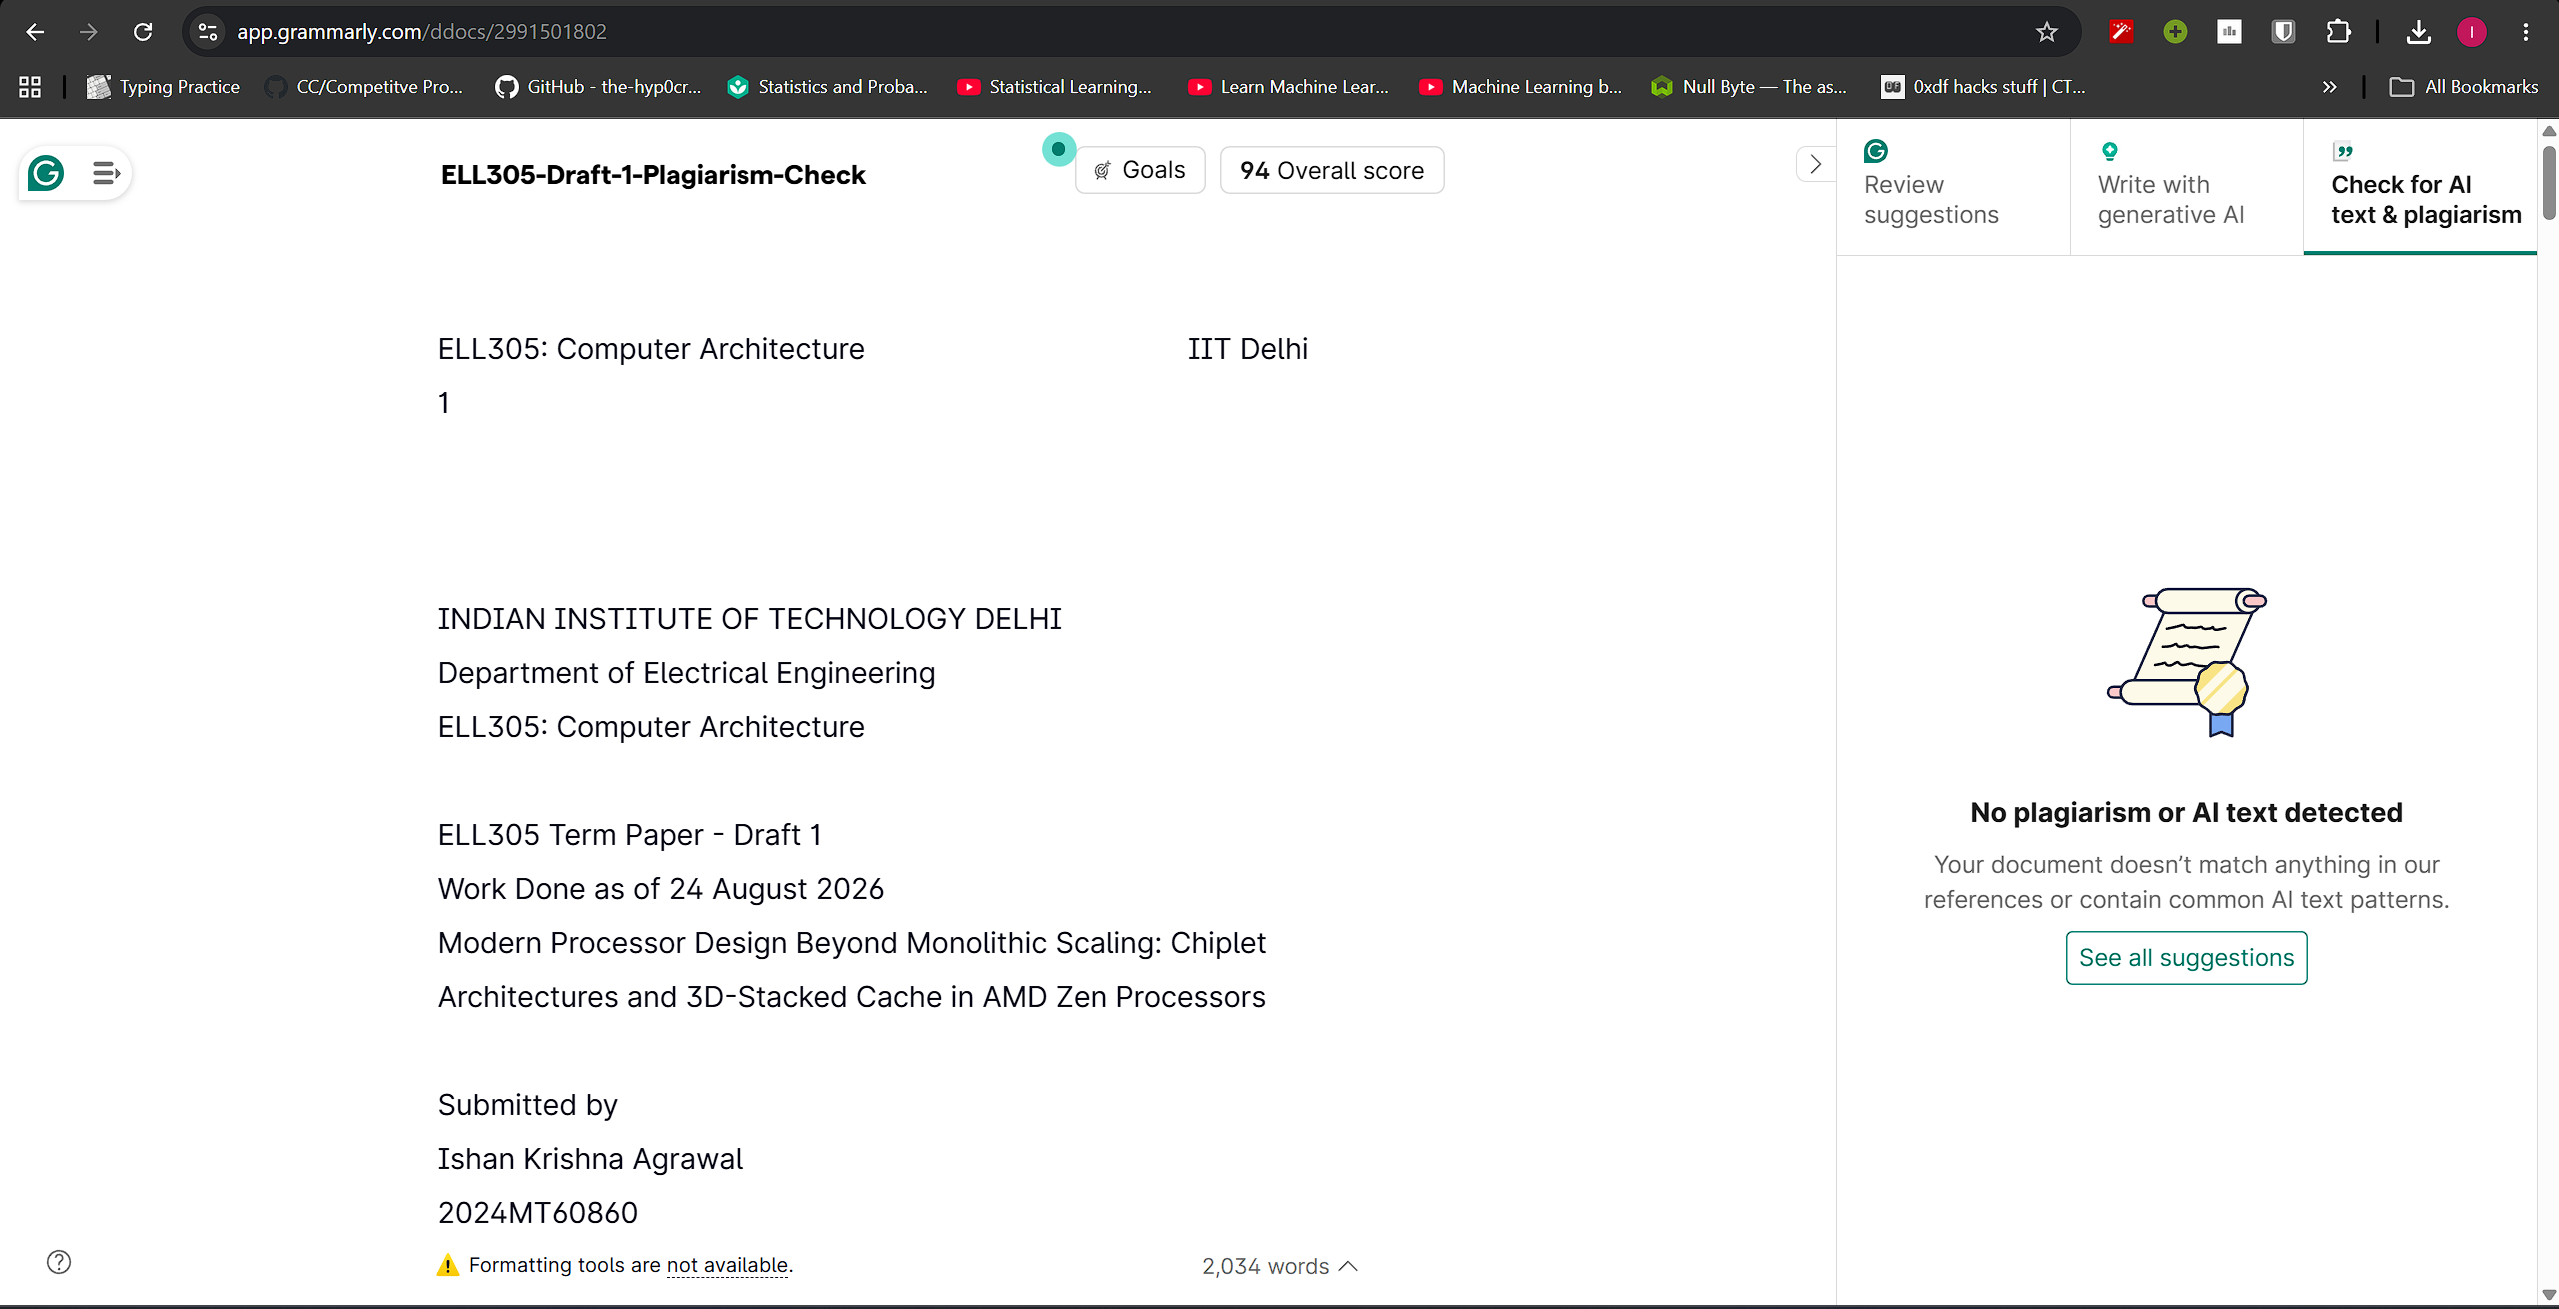
\includegraphics[width=0.96\textwidth]{grammarly-plagiarism-report-2026-08-24.png}
  \caption{Grammarly result displayed for the Draft 1 plagiarism-check copy on 24 August 2026.}
  \label{fig:plagiarism-result}
\end{figure}

% ==================== APPENDIX B - READING INDICES ====================
\clearpage
\section{Reading Indices}
\label{app:reading-indices}
\index{readability indices}

The readability analysis supplied for the Draft~1 plagiarism-check text reported the grade-level estimates shown in Table~\ref{tab:reading-indices}. The values are reproduced exactly as displayed by the analysis tool.

\begin{table}[htbp]
    \centering
    \caption{Reading indices reported for Draft~1}
    \label{tab:reading-indices}
    \begin{tabular}{@{}lr@{}}
        \toprule
        \textbf{Reading index} & \textbf{Grade-level estimate} \\
        \midrule
        Gunning Fog & 17.99 \\
        Flesch--Kincaid Grade Level & 15.26 \\
        SMOG & 15.84 \\
        Coleman--Liau & 19.82 \\
        Automated Readability Index & 17.92 \\
        \midrule
        Average grade level & 17.37 \\
        Median grade level & 17.92 \\
        \bottomrule
    \end{tabular}
\end{table}

Taken together, these estimates indicate that the current report uses language associated with advanced undergraduate to graduate or professional reading levels. This is plausible for a technical computer-architecture report, in which specialised terminology and long technical expressions increase formula-based scores. The indices estimate linguistic complexity only; they do not measure technical correctness, writing quality, originality, or the strength of the argument. The interpretation follows the general description of readability measures provided by the analysis site.\footnote{\url{https://www.analyzemywriting.com/readability_indices.html}}

\begin{figure}[htbp]
    \centering
    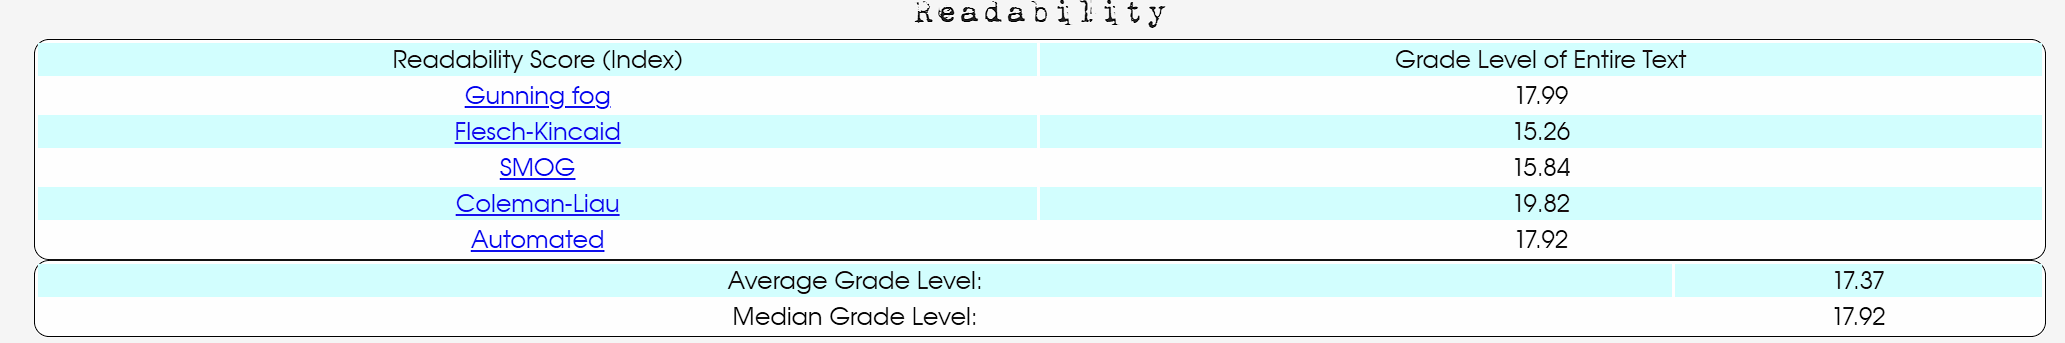
\includegraphics[width=0.98\textwidth]{readability-indices-2026-08-24.png}
    \caption{Readability-index results supplied for the Draft~1 text on 24 August 2026.}
    \label{fig:reading-indices-result}
\end{figure}

\clearpage

\phantomsection

\addcontentsline{toc}{section}{Index}

\setlength{\columnsep}{24pt}

\printindex

\end{document}
